\section{Solução Proposta}

\subsection{O que será automatizado?}

O processo de fabricação da cerveja exige um fino controle de variáveis do sistema tal como temperatura, tempo e nível dos líquidos. Assim sendo, a produção de cerveja artesanal esbarra em dificuldades de controle os quais podem ser resolvidos com a ajuda da engenharia, automatizando processos e etapas inteiras da produção da cerveja. Cada etapa da produção possui temperatura específica, que pode variar de acordo com o tipo de cerveja, e outras variáveis que devem ser mantidas constantemente sob controle para que o produto final tenha aspecto e a qualidade desejada.

A fim de se obter um maior controle de qualidade e facilidade na produção, as seguintes etapas são passíveis de serem monitoradas e controladas:

\subsubsection{Brassagem}
\begin{itemize}
    \item Aumentar a temperatura até chegar a 70 graus;
    \item Controlar a temperatura de 70 graus por determinado tempo;
    \item Aumentar a temperatura de 70 para 78 e manter;
    \item Adição do malte;
    \item Filtragem;
\end{itemize}

\subsubsection{Fervura}
\begin{itemize}
    \item Aumentar a temperatura de 78 para 100 graus;
    \item Adicionar o lúpulo;
    \item Controlar o tempo de fervura.
\end{itemize}


\subsubsection{Resfriamento}
\begin{itemize}
    \item Diminuir a temperatura para a temperatura ambiente;
    \item Filtragem do lúpulo;
    \item Oxigenação.
\end{itemize}


\subsubsection{Fermentação}
\begin{itemize}
    \item Adicionar a levedura;
    \item Teste de densidade;
    \item Liberar co2 sem receber o2.
\end{itemize}

As imagens a seguir ilustram as temperaturas dos processos e as ações que devem ser tomadas em cada etapa.

\begin{figure}[h]
    \centering
    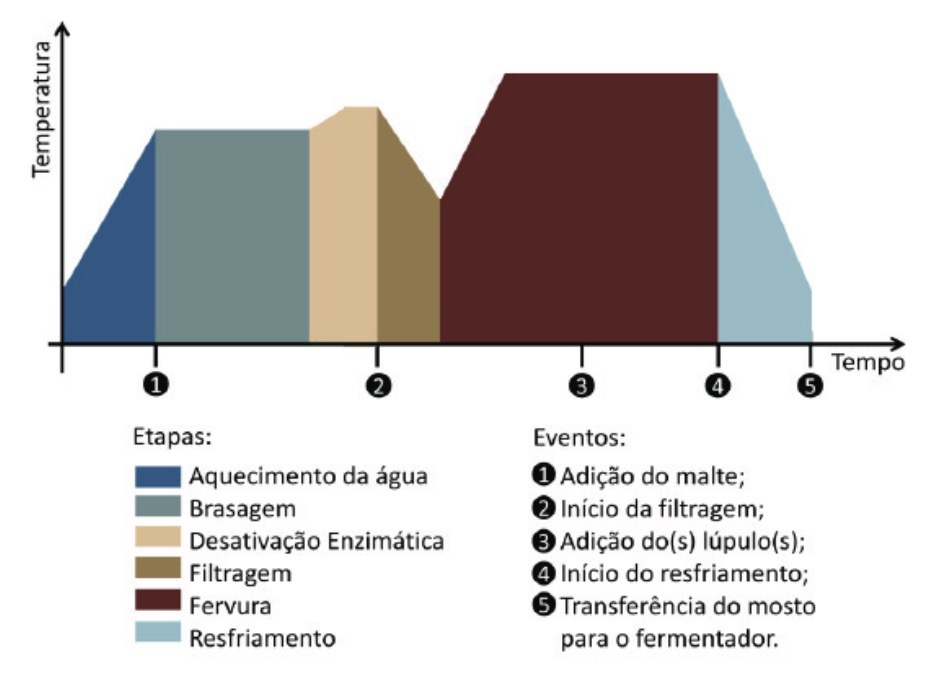
\includegraphics[scale=0.2]{images/grafico1.png}
    \caption{Eventos ao longo do tempo}
\end{figure}

\begin{figure}[h]
    \centering
    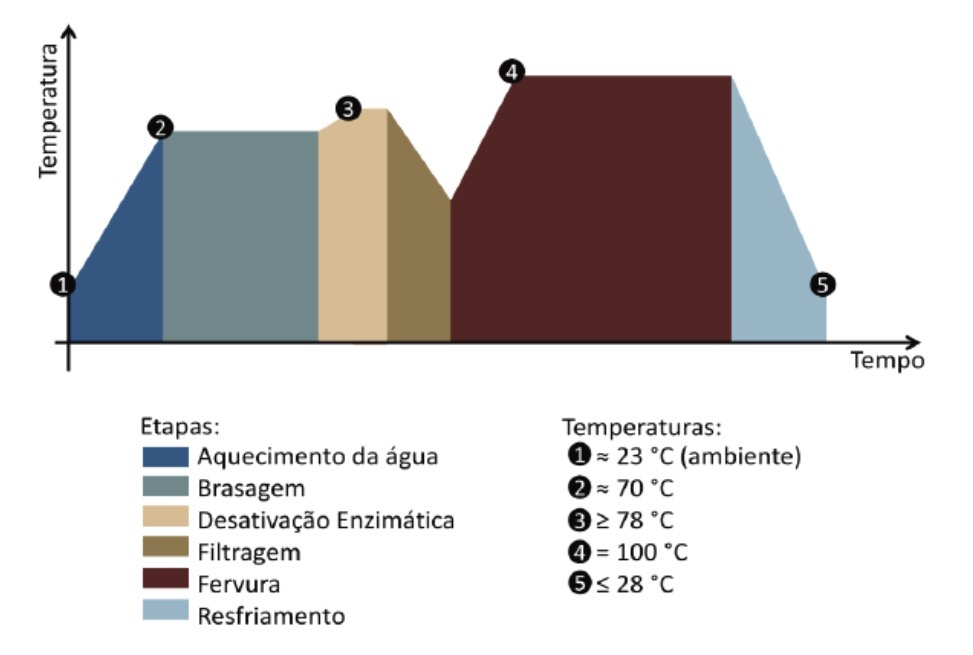
\includegraphics[scale=0.2]{images/grafico2.png}
    \caption{Temperaturas ao longo do tempo}
\end{figure}